\chapter{DATA PRE-PROCESSING}


\section{DATASET PRESENTATION:}
Creating a logistic regression for leads scoring (aka  conversion scoring ) needs a good dataset that represent the real data as a company could have . thus, we will use a dataset consists of various attributes such as Lead Source, Lead Origin, Total Visits, Last Activity, etc. which may or may not be useful in ultimately deciding whether a lead will be converted or not. The target variable, in this case, is the column ‘Converted’ which tells whether a past lead was converted or not wherein 1 means it was converted and 0 means it wasn’t converted.
\textbf{So: } the goal here is to Build a logistic regression model in R language to assign a lead score between 0 and 100 to each of the leads which can be used by the company to target potential leads. A higher score would mean that the lead is hot, i.e. is most likely to convert whereas a lower score would mean that the lead is cold and will mostly not get converted.\\
So without further to do lets dive in.\\
\textbf{\large Data loading: }\\
First we can load our dataset from a csv file using this command .
\begin{lstlisting}[language=R]
> leads_data = read.csv(leads.csv")
\end{lstlisting}
\begin{figure}[ht]
    \centering
    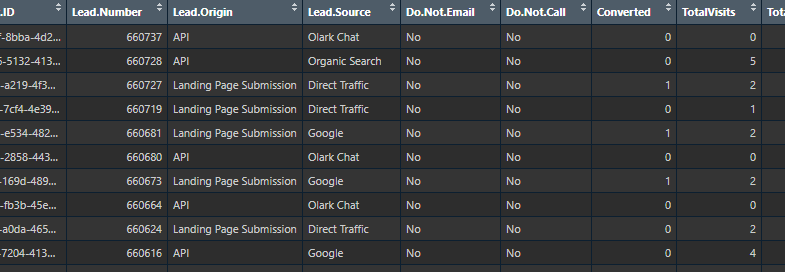
\includegraphics[width=0.8\textwidth]{assets/leadsData.png}
    \caption{ Leads dataset}
\end{figure}
we can check whether a dataset contain a duplicated values like so .
\begin{lstlisting}[language=R]
> sum(duplicated(leads_data)) == 0 # True => No duplicate values
[1] TRUE
\end{lstlisting}
\textbf{\large Data Inspection: }\\
By dimension we mean the number of rows and columns represented in the dataset . 
\begin{lstlisting}[language=R]
> dim(leads_data)
[1] 9240   37
\end{lstlisting}
we could see a lot of information about our dataset just by using the summary() method .  
\begin{lstlisting}[language=R]
> summary(leads_data)
 Prospect.ID         Lead.Number     Lead.Origin        Lead.Source        Do.Not.Email      
 Length:9240        Min.   :579533   Length:9240        Length:9240        Length:9240       
 Class :character   1st Qu.:596485   Class :character   Class :character   Class :character  
 Mode  :character   Median :615479   Mode  :character   Mode  :character   Mode  :character  
                    Mean   :617188           
                    3rd Qu.:637387          
                    Max.   :660737                
                   ...
 \end{lstlisting}



\section{DATA CLEANING:}\\
data cleaning consist of removing or correcting the unused values and columns . Now we will see different cleaning processes on different attributes or what we call it in data science Features . 
For example here we replace the unused value "Select" in the column Specialization with NA ( which is a none value ) .
\begin{lstlisting}[language=R]
> leads_data$Specialization = ifelse(leads_data$Specialization == "Select",
                 NA,
                 leads_data$Specialization)
\end{lstlisting}
After this we need to know the NA frequency in each column to make a decision if this column is contain a significant information or not . 
\begin{lstlisting}[language=R]
> sum_na = sapply(leads_data, function(x) sum(is.na(x)))
> round(100*(sum_na/nrow(leads_data)), 2)
Prospect.ID                                     Lead.Number 
0.00                                            0.00 
Lead.Origin                                     Lead.Source 
0.00                                            0.00 
Do.Not.Email                                    Do.Not.Call 
0.00                                            0.00 
Converted                                       TotalVisits 
0.00                                            1.48 
Total.Time.Spent.on.Website                     Page.Views.Per.Visit 
0.00                                            1.48 
Last.Activity                                   Country 
0.00                                            0.00 
Specialization                                  How.did.you.hear.about.WISD 
21.02                                           0.00 
Search                                          Magazine 
0.00                                            0.00 
Newspaper.Article                               WISD..Forums 
0.00                                            0.00 

Asymmetrique.Activity.Score                     Asymmetrique.Profile.Score 
45.65                                           45.65 
\end{lstlisting}
For now we will drop the columns having more than 70\% NA values because it mean that the column doesn't represent any information and that is possible by using this for loop :
\begin{lstlisting}[language=R]
> for( i in 0:ncol(leads_data)){
+   sum_col_na = sum(is.na(leads_data[i]))
+   na_percentage = round(100*(sum_col_na/nrow(leads_data)), 2)
+   print(na_percentage)
+   if( na_percentage > 70){
+     leads_data = subset(leads_data, select = -c(i)) #select(leads_data, i)
+   }
+ }
\end{lstlisting}
Now we will take care of empty values in each column one by one.
\begin{lstlisting}[language=R]
> leads_data[leads_data == ""] = NA
\end{lstlisting}
\textbf{Lead Quality: }\\
Indicates the quality of lead based on the data and intuition the employee who has been assigned to the lead
\begin{lstlisting}[language=R]
> describe(leads_data$Lead.Quality)
leads_data$Lead.Quality 
       n  missing distinct 
    4473     4767        5 

lowest : High in Relevance Low in Relevance  Might be          Not Sure          Worst            
highest: High in Relevance Low in Relevance  Might be          Not Sure          Worst            
                    
Value      High in Relevance  Low in Relevance          Might be          Not Sure             Worst
Frequency                637               583              1560              1092               601
Proportion             0.142             0.130             0.349             0.244             0.134
\end{lstlisting}
There is too much variation in these parameters so its not reliable to impute any value in it.
\begin{lstlisting}[language=R]
> ggplot(leads_data, aes(x=reorder(leadQuality, leadQuality, function(x)-length(x)))) +
+ geom_bar(fill='red') +  labs(x='leads Quality')
\end{lstlisting}
\begin{figure}[ht]
    \centering
    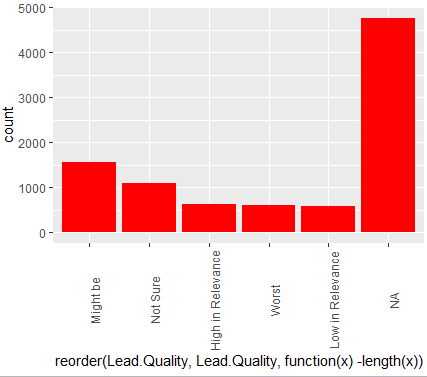
\includegraphics[width=0.5\textwidth]{assets/lead_quality.png}
    \caption{ Leads Quality Bar plot}
\end{figure}
 So as Lead quality is based on the intuition of employee, so if left blank we can impute 'Not Sure' in NA safely.
\begin{lstlisting}[language=R]
> leads_data$Lead.Quality = ifelse( is.na( leads_data$Lead.Quality ),"Not Sure",leads_data$Lead.Quality)
> ggplot(leads_data, aes(x=reorder(leadQuality, leadQuality, function(x)-length(x)))) +
+ geom_bar(fill='red') +  labs(x='leads Quality')
\end{lstlisting}
\begin{figure}[ht]
    \centering
    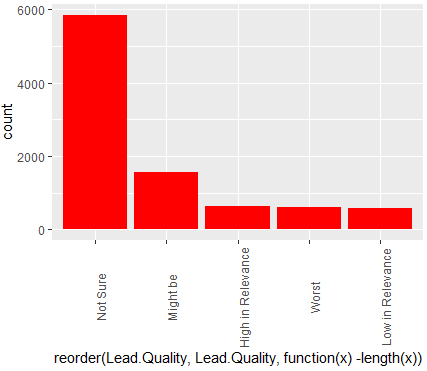
\includegraphics[width=0.5\textwidth]{assets/lead_quality2.png}
    \caption{ Leads Quality Bar plot}
\end{figure}
\textbf{Leads Asymmetrique: }\\
An index and score assigned to each customer based on their activity and their profile . and we can visualize their variations from this graphs : 
\begin{lstlisting}[language=R]
> as_act_score = leads_data$Asymmetrique.Activity.Score 
> ggplot(leads_data, aes(x=reorder(as_act_score, as_act_score, function(x)-length(x))))
+   geom_bar(fill='red') +  labs(x='Asymmetrique.Activity.Score')
> ggplot(leads_data, aes(x=as_act_score, y=as_act_score ) )+
+   geom_boxplot(fill='steelblue') +  labs(x='Asymmetrique.Activity.Score') +coord_flip()
> as_prf_indx = leads_data$Asymmetrique.Profile.Index 
> ggplot(leads_data, aes(x=reorder(as_prf_indx, as_prf_indx, function(x)-length(x)))) +
+   geom_bar(fill='red') +  labs(x='Asymmetrique.Activity.Score')
> as_prf_score = leads_data$Asymmetrique.Profile.Score
> ggplot(leads_data, aes(x=as_prf_score, y=as_prf_score ) )+
+   geom_boxplot(fill='steelblue') +  labs(x='Asymmetrique.Activity.Score') + coord_flip()
\end{lstlisting}
\begin{figure}[H]
	\begin{center}
		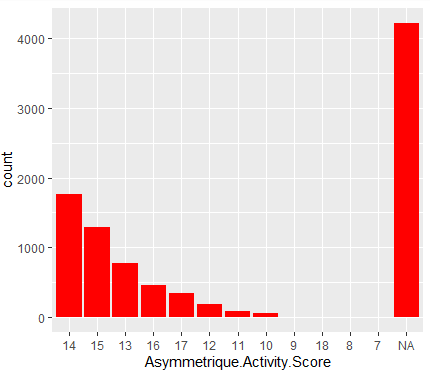
\includegraphics[width=0.41\textwidth]{assets/score_activ.PNG}	
		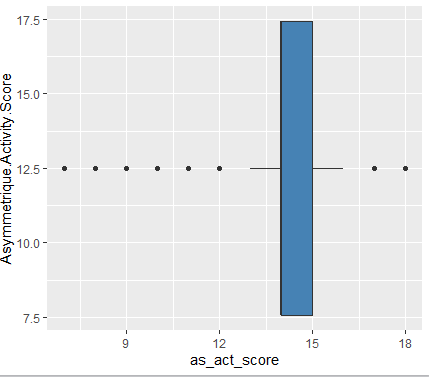
\includegraphics[width=0.41\textwidth]{assets/as_score.PNG}
	\end{center}
	\begin{center}
		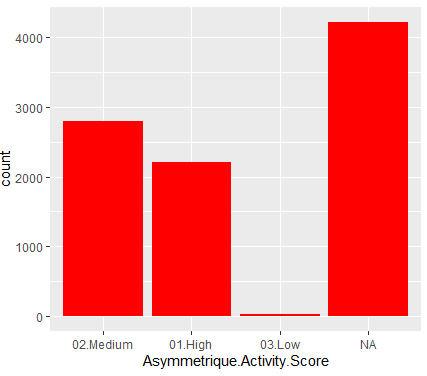
\includegraphics[width=0.41\textwidth]{assets/profil_score.PNG}	
		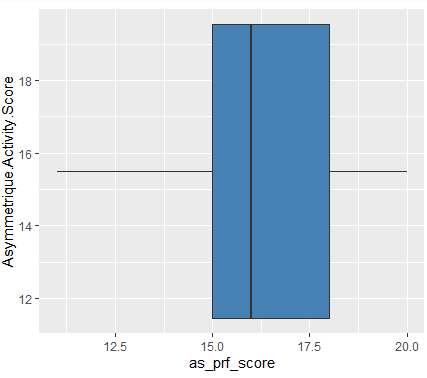
\includegraphics[width=0.41\textwidth]{assets/as_pr_score.PNG}
	\end{center}
\end{figure}
\textbf{City: }\\
This is the city related to the user profile .
\begin{lstlisting}[language=R]
> describe(leads_data$City)
leads_data$City 
       n  missing distinct 
    7820     1420        7 
lowest : Mumbai                      Other Cities                Other Cities of Maharashtra Other Metro Cities          Select             
highest: Other Cities of Maharashtra Other Metro Cities          Select                      Thane & Outskirts           Tier II Cities             
Mumbai (3222, 0.412), Other Cities (686, 0.088), Other Cities of Maharashtra (457, 0.058),
Other Metro Cities (380, 0.049), Select (2249, 0.288), Thane & Outskirts (752, 0.096), Tier II
Cities (74, 0.009)
\end{lstlisting}
\begin{lstlisting}[language=R]
> ggplot(leads_data, aes(x=reorder(City, City, function(x)-length(x)))) +
+   geom_bar(fill='red') +  labs(x='City', y="") + 
+   theme(axis.text.x = element_text(angle = 90))
\end{lstlisting}
\begin{figure}[H]
    \centering
    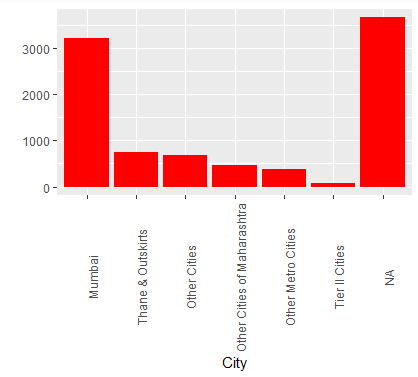
\includegraphics[width=0.5\textwidth]{assets/city.png}
    \caption{ City BarPlot}
\end{figure}
Around 60\% of the data is Mumbai so we can impute Mumbai in the missing values (NA or Select).
\begin{lstlisting}[language=R]
> leads_data$City = ifelse(is.na(leads_data$City),"Mumbai",leads_data$City)
> leads_data$City = ifelse(leads_data$City == "Select","Mumbai",leads_data$City)
\end{lstlisting}
\textbf{Specailization}\\
This column specifies the specialization domain of the lead ( i.e the specialization of the user that represent this lead ).
\begin{lstlisting}[language=R]
> describe(leads_data$Specialization)
leads_data$Specialization 
       n  missing distinct 
    5860     3380       18 

lowest : Banking, Investment And Insurance Business Administration           E-Business                        E-COMMERCE       Finance Management               
highest: Retail Management                 Rural and Agribusiness            Services Excellence               Supply Chain Management Travel and Tourism 
> ggplot(leads_data, aes(x=reorder(Specialization, Specialization, function(x)-length(x)))) +
+   geom_bar(fill='red') +  labs(x='Specialization', y="") + 
+   theme(axis.text.x = element_text(angle = 90))
\end{lstlisting}
\begin{figure}[H]
    \centering
    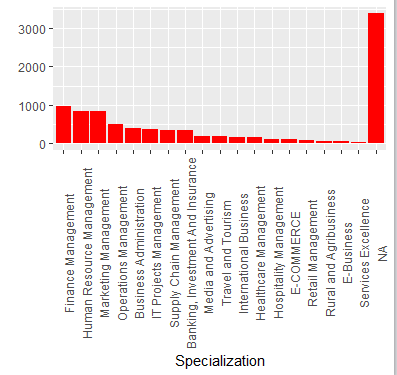
\includegraphics[width=0.5\textwidth]{assets/specialisation.png}
    \caption{ Specialization BarPlot}
\end{figure}
It maybe the case that lead has not entered any specialization if his/her option is not available on the list, may not have any specialization or is a student , Hence we can make a category "Others" for missing values.
\begin{lstlisting}[language=R]
> leads_data$Specialization = ifelse(is.na(leads_data$Specialization),"Others",leads_data$Specialization)
\end{lstlisting}
\textbf{Tags: }\\
Tags are able to determine some extra information about the user .
\begin{lstlisting}[language=R]
> describe(leads_data$Tags)
leads_data$Tags 
       n  missing distinct 
    5887     3353       26 

lowest : Already a student                                 Busy                                              Closed by Horizzon                                Diploma holder (Not Eligible)                     Graduation in progress                           
highest: switched off                                      University not recognized                         Want to take admission but has financial problems Will revert after reading the email               wrong number given
\end{lstlisting}
Blanks in the tag column may be imputed by 'Will back after reading the email'.
\begin{lstlisting}[language=R]
> leads_data$Tags = ifelse(is.na(leads_data$Tags),"Will back after reading the email",leads_data$Tags)
\end{lstlisting}
\textbf{Occupation: }\\
Occupation are able to dusting the occupation of the user (could represent work, job, activity, etc..) .
\begin{lstlisting}[language=R]
> describe(leads_data$What.is.your.current.occupation)
leads_data$What.is.your.current.occupation 
       n  missing distinct 
    6550     2690        6 

lowest : Businessman          Housewife            Other                Student              Unemployed          
highest: Housewife            Other                Student              Unemployed           Working Professional
Value               Businessman            Housewife                Other              Student           Unemployed
Frequency                     8                   10                   16                  210                 5600
Proportion                0.001                0.002                0.002                0.032                0.855
                               
Value      Working Professional
Frequency                   706
Proportion                0.108
\end{lstlisting}
We can see from the proportion row that 86\% entries are of Unemployed so we can impute "Unemployed" in it .
\begin{lstlisting}[language=R]
> leads_data$What.is.your.current.occupation = ifelse(is.na(leads_data$What.is.your.current.occupation),"Unemployed",leads_data$What.is.your.current.occupation)
\end{lstlisting}
This is the most important cleaning parts the same work is done for the other columns such as exploring , replacing, and finally cleaning . So we continue the same work on all the dataset until Data will be cleaned to start with the analysis part .\\



\section{DATA ANALYTIC:}\\
\textbf{\large Univariate Analysis: }\\
\textbf{Converted: }\\
Converted is the target variable, Indicates whether a lead has been successfully converted (1) or not (0) , So lets explore it first .
\begin{lstlisting}[language=R]
> convertedFreq = (sum(leads_data$Converted)/length(leads_data$Converted))*100
> convertedFreq
[1] 38.53896
\end{lstlisting}
\textbf{Lead Origin: }
\begin{lstlisting}[language=R]
> ggplot(leads_data) + geom_bar(aes(x = Lead.Origin, fill = as.factor(Converted)), position = "dodge") + theme(axis.text.x = element_text(angle = 90))
\end{lstlisting}
\begin{figure}[H]
    \centering
    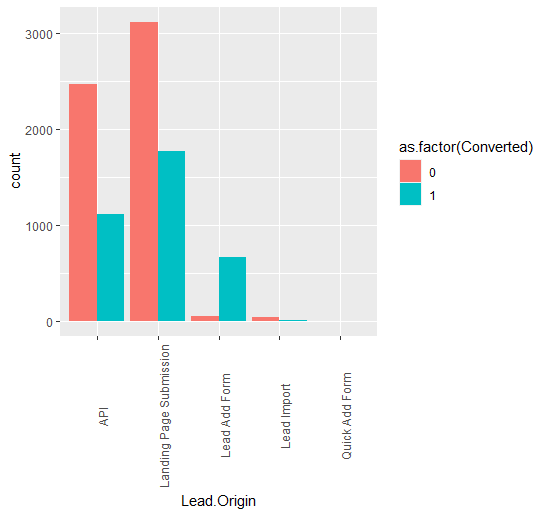
\includegraphics[width=0.5\textwidth]{assets/origin.png}
    \caption{ Leads dataset}
\end{figure}
The values API and Landing Page Submission have 30-35\% conversion rate but count of lead originated from them are considerable.
And the value Lead Add Form has more than 90\% conversion rate but count of lead are not very high.
In the other hand Lead Import are very less in count.
To improve overall lead conversion rate, we need to focus more on improving lead conversion of API and Landing Page Submission origin and generate more leads from Lead Add Form.
\textbf{Lead Source: }
\begin{lstlisting}[language=R]
> ggplot(leads_data) +geom_bar(aes(x = Lead.Source, fill = as.factor(Converted)), position = "dodge") + theme(axis.text.x = element_text(angle = 90))
\end{lstlisting}
\begin{figure}[H]
    \centering
    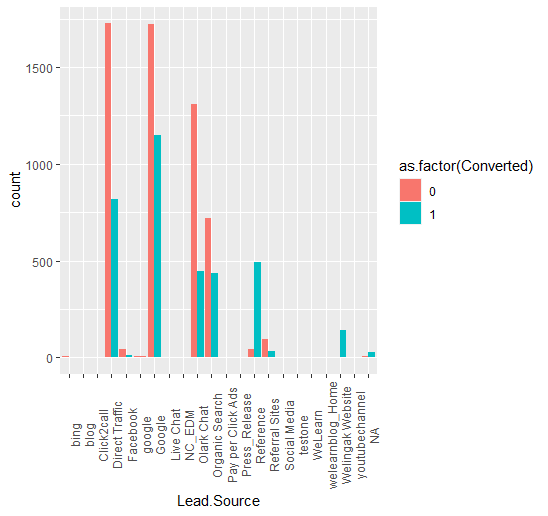
\includegraphics[width=0.5\textwidth]{assets/source.png}
    \caption{ Leads dataset}
\end{figure}
\begin{lstlisting}[language=R]
> leads_data$Lead.Source = ifelse( leads_data$Lead.Source == "google","Google",leads_data$Lead.Source)
> leads_data$Lead.Source = ifelse( is.na(leads_data$Lead.Source == "google"),"Others",leads_data$Lead.Source)
> leads_data$Lead.Source = ifelse( leads_data$Lead.Source %in% c('Click2call', 'Live Chat', 'NC_EDM', 'Pay per Click Ads', 'Press_Release','Social Media', 'WeLearn', 'bing', 'blog', 'testone', 'welearnblog_Home', 'youtubechannel'),"Others",leads_data$Lead.Source)
> ggplot(leads_data) + geom_bar(aes(x = Lead.Source, fill = as.factor(Converted)), position = "dodge") + theme(axis.text.x = element_text(angle = 90))
\end{lstlisting}
\begin{figure}[H]
    \centering
    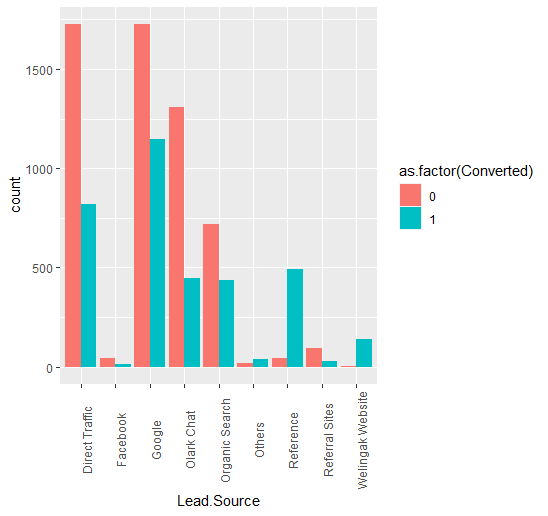
\includegraphics[width=0.5\textwidth]{assets/s.png}
    \caption{ Leads dataset}
\end{figure}
From this plot we can make some inferences like so .
Google and Direct traffic generates maximum number of leads.
Conversion Rate of reference leads and leads through welingak website is high.
To improve overall lead conversion rate, focus should be on improving lead conversion of olark chat, organic search, direct traffic, and google leads and generate more leads from reference and welingak website.\\
\textbf{Do Not Email & Do Not Call: }\\
These two columns contain Yes or No .  
\begin{lstlisting}[language=R]
> ggplot(leads_data) +geom_bar(aes(x = Do.Not.Call, fill = as.factor(Converted)), position = "dodge") + theme(axis.text.x = element_text(angle = 90))
> ggplot(leads_data) +geom_bar(aes(x = Do.Not.Email, fill = as.factor(Converted)), position = "dodge") + theme(axis.text.x = element_text(angle = 90))
\end{lstlisting}
\begin{figure}[H]
	\begin{center}
		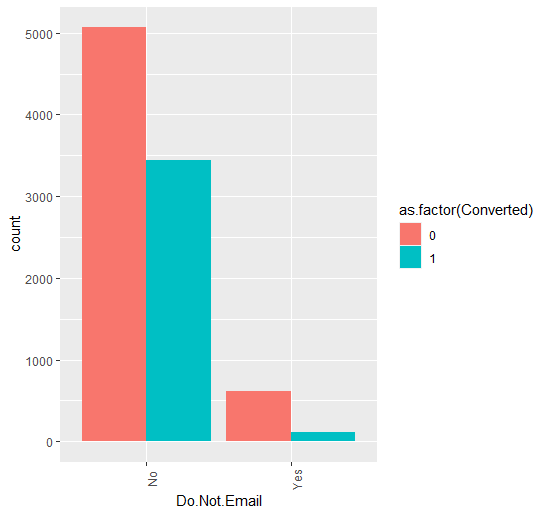
\includegraphics[width=0.41\textwidth]{assets/email.png}	
		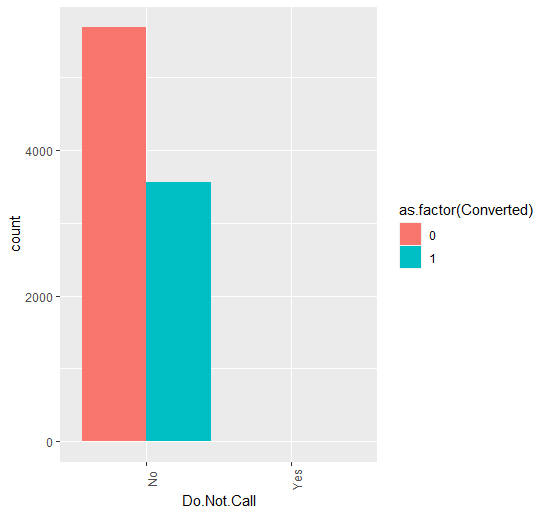
\includegraphics[width=0.41\textwidth]{assets/call.png}
	\end{center}
\end{figure}
\textbf{Total Visits: }\\
We can say that TotalVisits represent the engaging rate of the users , so a higher visits mean a higher possibility to convert . 
\begin{lstlisting}[language=R]
> ggplot(leads_data, aes(x=TotalVisits, y=TotalVisits ) )+ geom_boxplot(fill='steelblue') +  labs(x='TotalVisits') + coord_flip()
\end{lstlisting}
\begin{figure}[H]
		\centering
    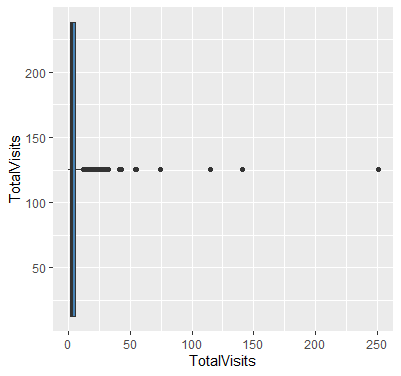
\includegraphics[width=0.5\textwidth]{assets/visit.png}
    \caption{Total Visits barplot}	
\end{figure}
As we can see there are a number of outliers in the data.
We will cap the outliers to 95\% value for analysis.
\begin{lstlisting}[language=R]
> fun <- function(x){
+   quantiles <- quantile( x, c(.05, .95 ), na.rm = T )
+   x[ x <= quantiles[0] ] <- quantiles[0]
+   x[ x >= quantiles[1] ] <- quantiles[1]
+   x
+ }
> leads_data$TotalVisits <- squish(leads_data$TotalVisits, quantile(leads_data$TotalVisits, c(.05, .95), na.rm = T))
> ggplot(leads_data, aes(x=Converted, y=TotalVisits ) )+
+   geom_boxplot(fill='steelblue') +  labs(x='TotalVisits') + coord_flip()
\end{lstlisting}
\begin{figure}[H]
		\centering
    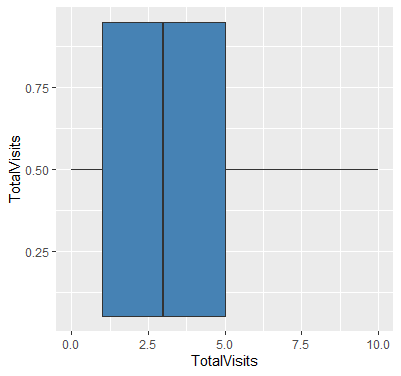
\includegraphics[width=0.5\textwidth]{assets/visi.png}
    \caption{Total Visits}	
\end{figure}

\begin{lstlisting}[language=R]
> ggplot(leads_data, aes(x = Converted, y = TotalVisits, fill=factor(Converted))) +
+   geom_boxplot() 
\end{lstlisting}
\begin{figure}[H]
		\centering
    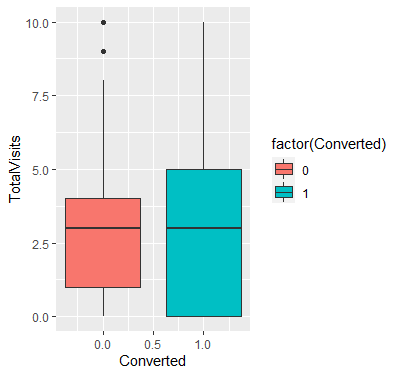
\includegraphics[width=0.5\textwidth]{assets/conn.png}
    \caption{Total Visits converted}	
\end{figure}
Here we see that Median for converted and not converted leads are the same . Which mean nothing conclusive can be said on the basis of Total Visits.
\textbf{Total time spent on website: }
\begin{lstlisting}[language=R]
> ggplot(leads_data, aes(x = Converted, y = Total.Time.Spent.on.Website, fill=factor(Converted))) + geom_boxplot()
\end{lstlisting}
\begin{figure}[H]
		\centering
    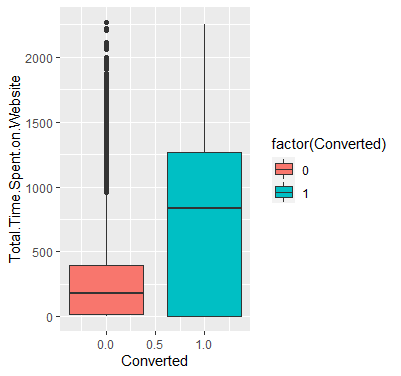
\includegraphics[width=0.5\textwidth]{assets/time.png}
    \caption{Total Visits converted}	
\end{figure}
We remark that Leads spending more time on the weblise are more likely to be converted. and Website should be made more engaging to make leads spend more time.

we apply  the same processing on all the dataset and we get this conclusion from the result of each study:

\begin{enumerate}
\item Nothing can be said specifically for lead conversion from Page Views Per Visit
\item Most of the lead have their Email opened as their last activity.
\item Conversion rate for leads with last activity as SMS Sent is almost 60%
\item Most values are 'India'  so no such inference can be drawn in country
\item Focus should be more on the Specialization with high conversion rate.
\item Working Professionals going for the course have high chances of joining it.
\item Unemployed leads are the most in numbers but has around 30-35\% conversion rate.
\item Most entries are 'Better Career Prospects'. No Inference can be drawn with this parameter.
\item Most entries are 'No' so no inference can be drawn with these parameters (search, Magazine, Newspaper Article,WISD Education Forums, Newspaper, Newspaper, Through Recommendations, Receive More Updates About Our Courses, Update me on Supply Chain Content, Get updates on DM Content, I agree to pay the amount through cheque, A free copy of Mastering The Interview) 
\item Most leads are from mumbai with around 30\% conversion rate.
\end{enumerate}
\textbf{Recapitulate: }\\
Based on the uni-variant analysis we have seen that many columns are not adding any information to the model, hence we can drop them for further analysis .
\begin{lstlisting}[language=R]
> leads_data = subset(leads_data, select = -c(Lead.Number, What.matters.most.to.you.in.choosing.a.course, Search, Newspaper.Article, WISD.Forums,Newspaper,Digital.Advertisement, Through.Recommendations, Receive.More.Updates.About.Our.Courses, Update.me.on.Supply.Chain.Content,Get.updates.on.DM.Content, I.agree.to.pay.the.amount.through.cheque,A.free.copy.of.Mastering.The.Interview, Country))
> dim(leads_data)
[1] 9240   19
\end{lstlisting}



\section{DATA PREPARATION:}
In this part we will prepare our data for building the model .
The first step is converting some binary variables (Yes/No) to 1/0
\begin{lstlisting}[language=R]
> leads_data$Do.Not.Call <- ifelse(leads_data$Do.Not.Call=="Yes", 1, 0)
> leads_data$Do.Not.Email <- ifelse(leads_data$Do.Not.Email=="Yes", 1, 0)
\end{lstlisting}
For categorical variables with multiple levels, create dummy features (one-hot encoded) using these liens of code .
\begin{lstlisting}[language=R]
> X = subset(leads_data, select = -c(Prospect.ID))
> X = X[!duplicated(X),]
> X$TotalVisits = c(scale(X$TotalVisits, center = TRUE, scale = TRUE))
> X$Total.Time.Spent.on.Website = c(scale(X$Total.Time.Spent.on.Website, center = TRUE, scale = TRUE))
> X$Page.Views.Per.Visit = c(scale(X$Page.Views.Per.Visit, center = TRUE, scale = TRUE))
\end{lstlisting}

Until this point we can say that our data is ready for training part using the binomial logistic regression  model to be able to predict the conversion state and score the leads from 0 to 100. 



%%%%%%%%%%%%%%%%%%%%%%%%%%%%%%%%%%%%%%%%%%%%%%%%%%%%%%%




\chapter{MODEL BUILDING}
\newpage
\lettrine[findent=2pt]{\textbf{F}}irst we will deep dive in describing this model , if you are not interested in the first section you can passe directly to model implementation section ( number 2.2 ) and you will consider the method that creates the model as a black box, don't worry you will be fine and able to understand the other parts .
\section{LOGISTIC REGRESSION}
To understand the purpose and to make sure that all of us in the same road lets Take an example where we want to know if a student will succeed in the exam based on the hours of studying . The problem here is that we use a non-categorical variable to predict a binary one ( 0 or 1 , succeed or fail ). For that we need to use a probability concept where we can take the working hours and calculate the probability to succeed in the exam from 0 to 1 .
So we get the S-shaped curve ( see the figure ) . the shape of our probability where the y axis is the probability value goes from 0 to 1 and the x axis for the studying hours . 

\begin{figure}[ht]
    \centering
    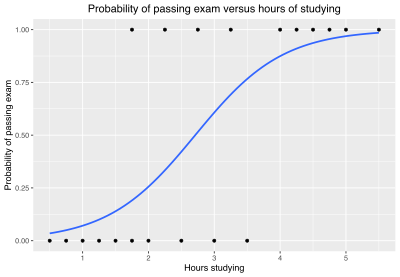
\includegraphics[width=0.5\textwidth]{assets/s-shape.png}
    \caption{ S-shape} 
    \label{fig:my_label}
\end{figure}
If we want to read this graph we could say the students that work for 2 hours have 25\% to succeed in the exams  and the students with 5 hours working rate are 95\% more likely to success in the exam ..etc.

This is one of the use cases where we want to find the correlation  between Y axis the probability of success and the studying hours .
Before , anything we need to present the model . so if you don't follow along in the mathematics part don't worry every will be getting more clear while reading . Lets deep dive in the mathematics . 
First we have the logistic function with this form :
\begin{align} 
\label{eq=Equation 1}  
Probability(Y = succeed | X = x,
a specific value of X) = \pi &= \frac{e^{\beta_0+\beta x}}{ {1+e^{\beta_0+\beta x}}}
\end{align}


$\pi$ is the probability to succeed in the exam , $\beta_0$ is the Y intercept , $\beta$ is the regression coefficient related to the variable X which can be categorical or continuous ,but Y is always categorical more specifically binary in the case of binary logistic regression .  

But curved shapes such a S-shaped , often referred to as sigmoidal , is difficult to describe with a linear equation for two reasons. First, the extremes do not follow a linear trend. Second, the errors are neither normally distributed nor constant across the entire range of data . Logistic regression solves these problems by applying the logit transformation to the dependent variable. In essence, the logistic model predicts the logit of Y from X. As stated earlier, the logit is the natural logarithm (ln) of odds of Y, and odds are ratios of probabilities ($\pi$) of Y happening ( i.e , a student is succeeded ) . Based on all of that , the simple logistic model has the form : 
\begin{align}
    logit(Y) = ln\left(\frac{\pi}{1-\pi}\right) = \beta_0 + \beta x
\end{align}

 According to Equation (1.2), the relationship between logit (Y) and X is linear. Yet, according to Equation (1.1), the relationship between the probability of Y and X is nonlinear. For this reason, the natural log transformation of the odds in Equation (1.2) is necessary to make the relationship between a categorical outcome variable and its predictor(s) linear.
 Extending the logic of the simple logistic regression to multiple predictors (say X1 = working hours and X2 = gender), one can construct a complex logistic regression for Y (recommendation for remedial reading programs) as follows:
 \begin{align*}
    &logit(Y) = ln\left(\frac{\pi}{1-\pi}\right) = {\beta_0 + \beta_1 x_1 + \beta_2 x_2 }\\
    &Therefore,\\
    &\pi = Probability (Y = outcome of interest | X_1 = x_1
, X_2 = x_2)\\  
    &= { \frac{e^{\beta_0 + \beta_1 x_1 + \beta_2 x_2}}{ {1+e^{\beta_0 + \beta_1 x_1 + \beta_2 x_2}}} }
\end{align*}
where $\pi$ is once again the probability of the success , $\beta_0$ is the Y intercept, $\beta _i$ are regression coefficients, and $X_i$ are a set of predictors. $\beta_0$ and $\beta _i$ are estimated by the maximum likelihood (ML) method  which is preferred over the weighted least squares approach .The ML method is designed to maximize the likelihood of reproducing the data given the parameter estimates ( we will deep dive on this method in the next chapter -chapter 2- ) .

Finally , we have the general logistic regression model as follow :
\begin{align*}
    &logit(Y) = ln\left(\frac{\pi}{1-\pi}\right) = {\beta_0 + \sum_{i=1}^n \beta_i x_i }\\
    &Therefore,\\
    &\pi = Probability ( Y = outcome of interest | X_1 = x_1, ..., X_n = x_n )\\  
    &= { \frac{e^{\beta_0 + \sum_{i=1}^n \beta_i x_i }}{ {1+e^{\beta_0 + \sum_{i=1}^n \beta_i x_i }}} }
\end{align*}
This is the logistic regression model a simple linear equation  between probability of success and a set of independent variables ( studying hours, gender ).  Now , you'd say yes this is the model a bunch of dummy parameter but how can I use it ? in other form , how can I train the model based on my dataset ? Good question,the model is a bunch of parameters needs to be calculated or estimated, Exactly that what we call it estimation , we can't define values from our heads, or making a magic function or formula that works for all datasets, but instead we find an estimated value for each parameter that depend on the dataset that we are using. And that what we will see in the next chapter.\\
\textbf{Parameters Estimation : }\\
To estimate the parameters in the logistic regression model we can’t minimize the residual sum of squares like was done in linear regression. Instead, we use a statistical technique called maximum likelihood. 
Before we dive into how the parameters of the model are estimated from data, we need to understand what logistic regression is calculating exactly .

This might be the most confusing part of logistic regression, so we will go over it slowly.

The equation for the standard logistic function is given by:
\begin{align*}
    f(z) = \frac{e^z}{1+e^z}
\end{align*}
The graph for this equation can be visualized as (\small{RMK: its similar to s-shaped figure} ).
\begin{figure}[ht]
    \centering
    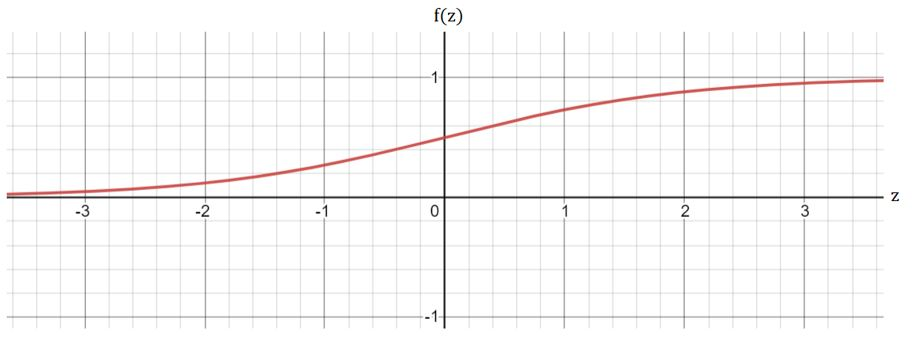
\includegraphics[width=0.5\textwidth]{assets/s-shaped2.jpg}
    \caption{ standard logistic equation } 
    \label{fig:my_label}
\end{figure}
In any proposed model, to predict the likelihood of an outcome, the variable z needs to be a function of the input or feature variables $X_1$, $X_2$,…, $X_n$. In logistic regression, z is often expressed as a linear function of the input variables as follows :
\begin{align*}
    &z  = {\beta_0 + \sum_{i=1}^n \beta_i x_i }\\
    &So, z = logit(Y) \\
    &keep it in mind .
\end{align*}
Suppose we have the data of n o    bservations ($y_1, y_2, …, y_n$) and ( $ x_1,x_2, …, x_n $ ). How do we estimate $\beta_0$ and $\beta_0$ ? Let’s first take a slight detour and take a very simple example using maximum likelihood estimation:\\
\textbf{\Large Coin Toss :}\\
The star of examples in statics world is coin toss . you don't hear about it .Okay here it is , suppose we have a coin, and we need to estimate the probability that it lands on the heads. Naturally, the first thing to do would be to toss it several times (say, n times) and note down the results (as binary outcomes: 1 for heads and 0 for tails). Suppose we record the observations as ($y_1, y_2, …, y_n$). We might then be tempted to find the sample mean of the observations and use it as an estimate for the probability of landing heads. So, if we get 3 heads and 7 tails in 10 tosses, we might conclude that the probability of landing heads is 0.3. Let’s see if we can use rigorous mathematics to confirm our intuition:

Let’s first identify the probability distribution of the coin toss example. Since the outcome variable is binary 0 and 1, it follows a Bernoulli distribution . 
The probability mass function of a Bernoulli distribution is
defined as:
\begin{align*}
    p(x) = \begin{cases}
                    &p,   y=1\\
                    &1-p, y=0 
            \end{cases}
\end{align*}
Often, the above function is simplified to a single line equation as follows:
\begin{align*}
    p(y) = p^y(1-p)^{(1-y)}
\end{align*}
We’ll now define the likelihood function for our distribution. In general, the likelihood function is defined as follows for discrete random variables as follows:
\begin{align*}
    L_n(Y_1,Y_2, ...,Y_n,\theta) = \mathbb{P}_\theta[Y_1=y_1,Y_2=y_2, ...,Y_n=y_n]
\end{align*}
Furthermore, while $Y_1, Y_2, …, Y_n$ are independent,
\begin{align*}
    &L_n(Y_1,Y_2, ...,Y_n,\theta) = \mathbb{P}_\theta[Y_1=y_1] \mathbb{P}_\theta[Y_2=y_2]...\mathbb{P}_\theta[Y_n=y_n]\\
    &\text{we define the probability mass function, for i in 1...n ,}\mathbb{P}_\theta[Y_i=y_i] = p(y_i)_\theta \\
    &L_n(Y_1,Y_2, ...,Y_n,\theta) = p_\theta[y_1] \mathbb{P}_\theta[Y_2=y_2]...\mathbb{P}_\theta[Y_n=y_n]
\end{align*}
Using this we can compute the likelihood function of the coin toss problem:
Parameter: $\theta$=p
Probability Mass Function:
\begin{align*}
    p_\theta(y) = p^y(y)(1-p)^{(1-y)}\\\\
\end{align*}
Likelihood function :
\begin{align*}
    L_n(Y_1,Y_2, ...,Y_n,\theta) = \prod_{i=1}^n  p_\theta[y_i] \\
\implies L_n(Y_1,Y_2, ...,Y_n,\theta) = p^{\sum y_i}(1-p)^{n-\sum y_i}
\end{align*}
Now that we have the likelihood function, we can easily find the maximum likelihood estimator (MLE) for the parameter p. The MLE  is defined as the value of $\theta$ that maximizes the likelihood function:
\begin{align*}
    \hat{\theta}^{MLE} = \underset{\theta\in\Theta}{argmax}\prod_{i=1}^n p_\theta[y_i]
    \\argmax return the parameter that maximize the likelihood function.
\end{align*}
Note
that $\Theta$ refers to the parameter space i.e., the range of values the unknown parameter $\theta$ can take. For our case, since p indicates the probability that the coin lands as heads, p is bounded between 0 and 1. Hence, $\theta$ = [0, 1]. We can use the tools of calculus to maximise the likelihood function. However, it’s often very tricky to take the derivatives. So, we use logarithmic differentiation by calculating the log-likelihood function and maximizing it instead of the likelihood function. Since log x is an increasing function,
\begin{align*}
    \hat{\theta}^{MLE} = \underset{\theta\in\Theta}{argmax}\prod_{i=1}^n p_\theta[y_i] = \underset{\theta\in\Theta}{argmax}\left[log\left(\prod_{i=1}^n p_\theta[y_i]\right)\right]
\end{align*}

Now that we’re equipped with the tools of maximum likelihood estimation, we can use them to find the MLE for the parameter p of Bernoulli distribution :
\begin{align*}
    log(L_n(Y_1,Y_2, ...,Y_n,p) &= log(p^{\sum y_i}(1-p)^{n-\sum y_i})\\
    &= \sum_{i=1}^n y_i log(p) + \left( n - \sum_{i=1}^n y_i\right)log(1-p)
\end{align*}
Maximum Likelihood Estimator:
\begin{align*}
    \boxed{\hat{\theta}^{MLE} = \hat{p}^{MLE} = \underset{\theta\in\Theta}{argmax}\left[ \sum_{i=1}^n y_i log(p) + \left( n - \sum_{i=1}^n y_i\right)log(1-p)\right]}
\end{align*}
Calculation of the First derivative:
\begin{align*}
    \frac{\partial}{\partial\theta}[log(L_n(Y_1,Y_2, ...,Y_n,\theta)] &= \frac{\partial}{\partial p}\left[ \sum_{i=1}^n y_i log(p) + \left( n - \sum_{i=1}^n y_i\right)log(1-p)\right] \\&= \frac{\sum_{i=1}^n y_i}{p} - \frac{n-\sum_{i=1}^n y_i}{1-p}
\end{align*}
Calculation of Critical Points in (0, 1):
\begin{align*}
    &\frac{\partial}{\partial\theta}[log(L_n(Y_1,Y_2, ...,Y_n,\theta)] = 0\\
    &\implies\frac{\sum_{i=1}^n y_i}{p} - \frac{n-\sum_{i=1}^n y_i}{1-p} = 0 \implies \frac{\sum_{i=1}^n y_i}{p} = \frac{n-\sum_{i=1}^n y_i}{1-p} \\
    &\implies p = \frac{1}{n}\sum_{i=1}^n y_i
\end{align*}
Calculation of the Second derivative:
\begin{align*}
    \frac{\partial^2}{\partial\theta^2}[log(L_n(Y_1,Y_2, ...,Y_n,\theta)] = \frac{\partial}{\partial\theta}\left[ \frac{\sum_{i=1}^n y_i}{p} - \frac{n-\sum_{i=1}^n y_i}{1-p}\right] = -\frac{\sum_{i=1}^n y_i}{p^2} - \frac{n-\sum_{i=1}^n y_i}{(1-p)^2}
\end{align*}
Substituting the estimator we obtained earlier in the above expression, we obtain,
\begin{align*}
    -\frac{n^2\sum_{i=1}^n y_i}{(\sum_{i=1}^n y_i)^2}-\frac{n^2(n-\sum_{i=1}^n y_i)}{(n-\sum_{i=1}^n y_i)^2} = -\left( \frac{n^2}{\sum_{i=1}^n y_i} - \frac{n^2}{(n-\sum_{i=1}^n y_i)}\right) < 0
\end{align*}
Therefore, $p = \frac{1}{n}\sum y_i)$ is the maximiser of the log-likelihood.
Therefore,
\begin{align*}
    \hat{p}^{MLE} = \frac{1}{n}\sum_{i=1}^n y_i)
\end{align*}
Yes, the MLE is the sample-mean estimator for the Bernoulli distribution. Isn’t it amazing how something so natural as a simple intuition could be confirmed using rigorous mathematical formulation and computation! We can now use this method of MLE to find the regression coefficients of the logistic regression.
\\\textbf{\Large Using MLE for the Logistic Regression Model}

Let’s first attempt to answer a simple question: what the probability distribution for our problem is? Is it the logistic function that we talked about earlier? Nope. It’s again the Bernoulli distribution. The only difference from the previous case is that this time the parameter p (probability that Y = 1) is the output of the logistic function. The data that we have is inputted into the logistic function, which gives the output:
\begin{align*}
    p = P(Y=1|X) = { \frac{e^{\beta_0 + \beta_1 x_1}}{ {1+e^{\beta_0 + \beta_1 x_1}}} }
\end{align*}
We can make the above substitution in the probability mass function of a Bernoulli distribution to get:
\\Parameters: $\theta = [\beta_0, \beta_1]$
\\probability mass function :
\begin{align*}
    p(y) &= p^y(1-p)^{(1-y)} \\
    &= \left(\frac{e^{\beta_0+\beta x}}{ {1+e^{\beta_0+\beta x}}}\right)^y \left(1-\frac{e^{\beta_0+\beta x}}{ {1+e^{\beta_0+\beta x}}}\right)\\
    &= \frac{( e^{\beta_0+\beta x} )^y}{(1+e^{\beta_0+\beta x})^y(1+e^{\beta_0+\beta x})^1-y}\\
    &= \frac{e^{y(\beta_0+\beta x)}}{1+e^{\beta_0+\beta x}}
\end{align*}
Likelihood Function:
\begin{align*}
     L_n(Y_1,Y_2, ...,Y_n,\theta) = \prod_{i=1}^n  p_\theta[y_i]\\
     \implies L_n(Y_1,Y_2, ...,Y_n,\beta_0, \beta_1) = \prod_{i=1}^n\frac{e^{y_i(\beta_0+\beta x_i)}}{1+e^{\beta_0+\beta x_i}}
\end{align*}
Log-likelihood Function:
\begin{align*}
    log(L_n(Y_1,Y_2, ...,Y_n,\beta_0, \beta_1) ) &=log\left(\prod_{i=1}^n\frac{e^{y_i(\beta_0+\beta x_i)}}{}\right)\\
    &=\sum_{i=1}^n log\left(\frac{}{1+e^{\beta_0+\beta x_i}}\right)\\
    &= \sum_{i=1}^n e^{y_i(\beta_0+\beta x_i)} - \sum_{i=1}^n 1+e^{\beta_0+\beta x_i}\\
    &= \sum_{i=1}^n y_i(\beta_0+\beta x_i) - \sum_{i=1}^n 1+e^{\beta_0+\beta x_i}\\
\end{align*}
Now that we’re derived the log-likelihood function, we can use it to determine the MLE:\\
Maximum Likelihood Estimator:
\begin{align*}
    \boxed{\hat{\theta}^{MLE} = \underset{\beta_0, \beta_1 \in (-\infty, \infty)}{argmax}\left[ log(L_n(Y_1,Y_2, ...,Y_n,\beta_0, \beta_1) )\right]}
\end{align*}
Unlike the previous example, this time we have 2 parameters to optimise instead of just one. Thus, we’ll have to employ tools in the domain of multi-variable calculus (gradients and partial derivatives) to solve our problem. We maximize the multi-dimensional log-likelihood function as follows:
Computing the Gradient of the Log-likelihood:
\begin{align*}
    \nabla log(L_n(Y_1,Y_2, ...,Y_n,\beta_0, \beta_1) ) = \pcases{\frac{\partial}{\partial\beta_0}log(L_n(Y_1,Y_2, ...,Y_n,\beta_0, \beta_1)\\\frac{\partial}{\partial\beta_1}log(L_n(Y_1,Y_2, ...,Y_n,\beta_0, \beta_1)}\\
    \implies \nabla log(L_n(Y_1,Y_2, ...,Y_n,\beta_0, \beta_1) ) = \pcases{\frac{\partial}{\partial\beta_0}(\sum_{i=1}^n y_i(\beta_0+\beta x_i) - \sum_{i=1}^n 1+e^{\beta_0+\beta x_i})\\\frac{\partial}{\partial\beta_1}(\sum_{i=1}^n y_i(\beta_0+\beta x_i) - \sum_{i=1}^n 1+e^{\beta_0+\beta x_i})}\\
    \implies \nabla log(L_n(Y_1,Y_2, ...,Y_n,\beta_0, \beta_1) ) =\pcases{
    \sum_{i=1}^n y_i - \frac{e^{y_i(\beta_0+\beta x_i)}}{1+e^{\beta_0+\beta x_i}}\\ \sum_{i=1}^n x_i y_i - \sum_{i=1}^n \frac{x_i e^{\beta_0+\beta x_i} }{1+e^{\beta_0+\beta x_i}}}
\end{align*}
Setting the gradient equal to the zero vector, we obtain,
\begin{align*}
    \nabla log(L_n(Y_1,Y_2, ...,Y_n,\beta_0, \beta_1) ) = \pcases{0\\0}
    \implies \pcases{
    \sum_{i=1}^n y_i - \frac{e^{y_i(\beta_0+\beta_1 x_i)}}{1+e^{\beta_0+\beta_1 x_i}}\\ \sum_{i=1}^n x_i y_i - \sum_{i=1}^n \frac{x_i e^{\beta_0+\beta_1 x_i} }{1+e^{\beta_0+\beta_1 x_i}}} = \pcases{0\\0}
\end{align*}
On comparing the first element, we obtain:
\begin{align*}
    \sum_{i=1}^n y_i - \frac{e^{y_i(\beta_0+\beta_1 x_i)}}{1+e^{\beta_0+\beta_1 x_i}} = 0
\end{align*}
On comparing the second element, we obtain:
\begin{align*}
    \sum_{i=1}^n x_i y_i - \sum_{i=1}^n \frac{x_i e^{\beta_0+\beta_1 x_i} }{1+e^{\beta_0+\beta_1 x_i}} = 0
\end{align*}
Thus, we have obtained the maximum likelihood estimators for the parameters of the logistic regression in the form of a pair of equations. Note that, there is no closed-form solution for the estimators. The solutions to the above pair of equations can be computed using various mathematical algorithms e.g., the Newton Raphson algorithm.\\
\textbf{\Large Simple Example}\\
Finally, to make some more sense of all the math we did, let’s plug in some real numbers. Suppose we have the following data where $x_i$ is the studying hours for the student number i , and $ y_i $ indicates whether the student succeeded or not ,  To simplify the calculations and the analysis, we have considered the case for only 3 students:  
\begin{figure}[ht]
    \centering
    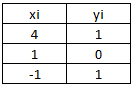
\includegraphics[width=0.2\textwidth]{assets/table1.png}
    \caption{ students and studying hours } 
\end{figure}
Let’s first use R to perform the calculations. We will then compare the results obtained by R with those obtained by using our equations:
\begin{lstlisting}[language=R]
    x <- c(4,1,-1)
    y <- c(1,0,1)
    fit <- glm(y ~ x, family = binomial(link = "logit"))
    coef(fit)
\end{lstlisting}
\begin{figure}[ht]
    \centering
    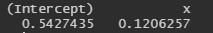
\includegraphics[width=0.3\textwidth]{assets/img1.png}
\end{figure}
Now, we’ll use the equations we derived:
\begin{align*}
    \sum_{i=1}^n y_i = 2 ; \sum_{i=1}^n x_i y_i = 4
\end{align*}
Thus, we have the following set of score equations:
\begin{align*}
    &2 - \frac{e^{(\beta_0+\beta_1 4)}}{1+e^{\beta_0+\beta_1 4}} - \frac{e^{(\beta_0+\beta_1 1)}}{1+e^{\beta_0+\beta_1 1}} - \frac{e^{(\beta_0+\beta_1 3)}}{1+e^{\beta_0+\beta_1 3}} = 0 \\
    &4 - \frac{4e^{(\beta_0+\beta_1 4)}}{1+e^{\beta_0+\beta_1 4}} - \frac{e^{(\beta_0+\beta_1 1)}}{1+e^{\beta_0+\beta_1 1}} + \frac{e^{(\beta_0-\beta_1 )}}{1+e^{\beta_0-\beta_1 }} = 0 
\end{align*}
We can plot the above equations to solve them graphically:
\begin{figure}[ht]
    \centering
    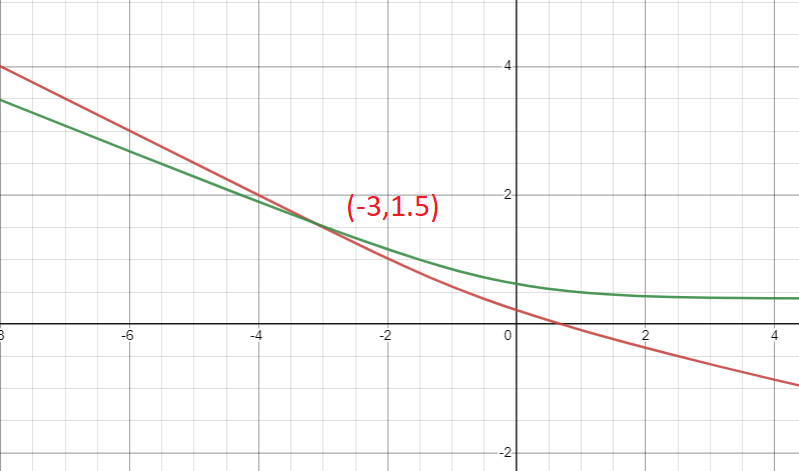
\includegraphics[width=0.5\textwidth]{assets/graph1.png}
\end{figure}
The intersection of the 2 graphs gives us the optimal value of the coefficients: (-3, 1.5). Voila! That’s incredibly close. Thus, we have been able to successfully use the tools of calculus and statistics to decode the computation processes that determine the coefficients of logistic regression.
Thus , our model is defined as follow :
\begin{align*}
    logit(Y) = ln\left(\frac{\pi}{1-\pi}\right) = -3 + 1.5 x\\
    &\text{Therefore, student that study 2 hours,}\\
    &\pi = Probability ( Y = outcome of interest | X=2 )\\  
    &= { \frac{e^{-3 + 1.5\times 2 }}{ {1+e^{-3 + 1.5\times 2 }}} }\\
    &= 1
\end{align*}

Create the model on simple data gives us a high accuracy easily but with complex data we need more than just a method, Lets get back to leads scoring and trying to apply all these concepts and if does it works or not . And see how we can improve our model and do what the WISD education needs from us.

\textbf{\Large Inference }
\newline
\textbf{R-Squared $R^2$}
\newline
the $R^2$ statistics measures the amount of variance explained by the regression model. The value of $R^2$ ranges in [0,1],with a larger value indicating more variance is explained by the model the values closer to 1 indicating better fit. 
For logistic regression, there have been many proposed pseudo-$R^2$
in this project we chose the methode of DL McFadden.
\begin{itemize}
\item DL McFadden stated that a pseudo-$R^2$ higher than 0.2 represents an excellent fit.
\item Additionally, McFadden’s $R^2$ can be negative.
\item these pseudo-$R^2$ values may be wildly different from one another.
\end{itemize}
\begin{align*}
R^2=1 - \frac{\ln({\hat{L_full}^{ }})}{\ln({\hat{L_null}^{ }})}
\end{align*}
\begin{itemize}
\item \(\hat{L_full}^{ }\)  is the estimated likelihood of the full model
\item \(\hat{L_null}^{ }\) is the estimated likelihood of the null model (model with only intercept)
\end{itemize}
\newline
\textbf{Score Test}


The score test relies on the fact that the slope of the log-likelihood function is 0 when \(\beta = \hat{\beta_j}^{ } \)
The idea is to evaluate the slope of the log-likelihood for the “reduced” model (does not include $\beta_1$) and see if it is “significantly” steep. The score test is also called Rao test. The test statistic, S, follows a  $\chi_r^2$ distribution when $H_0$ is true and n is large (r is the numnber of of variables set to zero, in this case = 1). The null hypothesis is rejected when S $>\chi_r^2(\alpha)$.

An advantage of the score test is that is only requires fitting the reduced model. This provides computational advantages in some complex situations (generally not an issue for logistic regression). Like the LRT, the score test doesn’t depend upon the model parameterization






%%%%%%%%%%%%%%%%%%%%%%%%%%%%%%%%%%%%%%%%%%%%%%%%%%%%%%%





\section{MODEL IMPLEMENTATION}  
Finally we are here in the most excited part in our project , now we will explore the magic of all this stuff , and see every thing in action.\\
So First lets checking the conversion rate to see if our data is balanced . 

\begin{lstlisting}[language=R]
> converted = (sum(leads_data$Converted/ length(leads_data$Converted)))*100
> converted
[1] 38.02043
\end{lstlisting}
as you see we have  almost 38\% conversion 
Next we split the dataset to 2 parts one for training(70\% of the dataset) and the others for test (30\% of the dataset)
\begin{lstlisting}[language=R]
set.seed(22)
sample <- createDataPartition(X$Converted, p = .7, list = F)
leads_data_train = X[sample, ]
leads_data_test = X[-sample, ]
\end{lstlisting}
Lets do it !! yes finally!! training the logistic regression model is here using this lines of code 
\begin{lstlisting}[language=R]
>logistic_reg <- glm(Converted~Do.Not.Email+Do.Not.Call+TotalVisits+Total.Time.Spent.on.Website+Page.Views.Per.Visit+Lead.OriginLanding.Page.Submission, family = "binomial", data = leads_data_train)
> summary(logistic_reg)

Call:
glm(formula = Converted ~ Do.Not.Email + Do.Not.Call + TotalVisits + 
    Total.Time.Spent.on.Website + Page.Views.Per.Visit + Lead.OriginLanding.Page.Submission, 
    family = "binomial", data = leads_data_train)

Deviance Residuals: 
    Min       1Q   Median       3Q      Max  
-2.2173  -0.8558  -0.6146   0.9635   2.4025  

Coefficients:
                                    Estimate Std. Error z value Pr(>|z|)    
(Intercept)                         -0.03442    0.05552  -0.620    0.535    
Do.Not.Email                        -1.18578    0.14148  -8.381  < 2e-16 ***
Do.Not.Call                         12.34464  190.43154   0.065    0.948    
TotalVisits                          0.06233    0.04233   1.472    0.141    
Total.Time.Spent.on.Website          0.94165    0.03408  27.632  < 2e-16 ***
Page.Views.Per.Visit                -0.24534    0.04551  -5.391 7.01e-08 ***
Lead.OriginLanding.Page.Submission  -0.55493    0.07115  -7.800 6.21e-15 ***
---
Signif. codes:  0 ‘***’ 0.001 ‘**’ 0.01 ‘*’ 0.05 ‘.’ 0.1 ‘ ’ 1

(Dispersion parameter for binomial family taken to be 1)

    Null deviance: 7067.1  on 5260  degrees of freedom
Residual deviance: 5965.6  on 5254  degrees of freedom
AIC: 5979.6

Number of Fisher Scoring iterations: 11
\end{lstlisting}
Yes this is our model as simple as it is, lets make some diagnostics .
\begin{lstlisting}[language=R]
> predict <- predict(logistic_reg, leads_data_test, type = 'response')
> table_mat <- table(leads_data_test$Converted, predict > 0.5)
> table_mat
    FALSE TRUE
  0  1185  208
  1   406  455

\end{lstlisting}
as you see the results show that 455 which is true positive and 1185 is false negative , it seems that something wrong here is our model working well ? .\\
Okay, lets check the accuracy of this model  
\begin{lstlisting}[language=R]
> accuracy_Test <- sum(diag(table_mat))/ sum(table_mat)  
> accuracy_Test
[1] 0.7275954
\end{lstlisting}
Oh ! here we go again why? how?
Don't worry I'm just kidding , unfortunately when we try to train the model using all columns it seems like some of them isn't a good predictor which make our model to generate wrong predictions, as you can see this model give 70\% in the accuracy .
but, what about R2 ?
there is no such R2 value for logistic regression ( for more details see the previous section in the estimation part ). Instead, we can compute a metric known as McFadden's R2, which ranges from 0 to just under 1. Values close to 0 indicate that the model has no predictive power. In practice, values over 0.40 indicate that a model fits the data very well.
We can compute McFadden's R2 for our model using the pR2 function from the pscl package:
\begin{lstlisting}[language=R]
> pscl::pR2(logistic_reg2)["McFadden"]
fitting null model for pseudo-r2
 McFadden 
0.159280
\end{lstlisting}
Here we are! our model doesn't fit the model.
This is why we need to make a decision about which column is a good predictor and which is not. That's possible using the RFE algorithm (Recursive Feature Elimination) , in the short form is a widely used algorithm for selecting features that are most relevant in predicting the target variable in a predictive model — either regression or classification.  
\begin{lstlisting}[language=R]
# This part of code take a lot of time to be executed 
> control_rfe = rfeControl(functions = rfFuncs, # random forest
                         method = "repeatedcv", # repeated cv
                         repeats = 5, # number of repeats
                         number = 10) # number of folds

> # Run RFE just while exploiting data
> result_rfe1 <- rfe(x = x_data_train,
                   y = y_data_train,
                   sizes = c(1:15),
                   rfeControl = control_rfe)

> # Print the selected features
> predictors(result_rfe1)
[1] "TagsWill.revert.after.reading.the.email"
[2] "TagsLost.to.EINS"
[3] "Total.Time.Spent.on.Website"
[4] "TagsClosed.by.Horizzon"
[5] "TagsRinging"
[6] "Last.Notable.ActivitySMS.Sent"
[7] "TagsWill.back.after.reading.the.email"
[8] "Last.Notable.ActivityModified"
[9] "Last.ActivitySMS.Sent"
[10] "Lead.QualityHigh.in.Relevance"
[11] "Lead.QualityNot.Sure"
[12] "TagsInterested.in.other.courses"
[13] "TagsBusy"
...
....
.....
[89] "Last.ActivityPage.Visited.on.Website"
[90] "SpecializationMarketing.Management"
[91] "CityOther.Cities"
[92] "SpecializationE.Business"
[93] "Last.Notable.ActivityPage.Visited.on.Website"
[94] "Last.ActivityOlark.Chat.Conversation"
\end{lstlisting}
We see that all columns are sorted in the way that the first are the best predictors and the last are the worst.
Based on this we can make another model on almost the same data but with less columns where we let just which seems the best from the RFE output.
\begin{lstlisting}[language=R]
logistic_reg2 <- glm(Converted~Do.Not.Email+Lead.OriginLead.Add.Form+
                       Lead.SourceWelingak.Website+
                       What.is.your.current.occupationWorking.Professional+TagsBusy+
                       TagsClosed.by.Horizzon+TagsLost.to.EINS+TagsRinging+
                       TagsWill.revert.after.reading.the.email+Tagsswitched.off+
                       Lead.QualityNot.Sure+Lead.QualityWorst+Last.Notable.ActivitySMS.Sent,
                     family = "binomial", data = leads_data_train)
\end{lstlisting}
With the same process as showing previously , we can show the accuracy and the R2, like so.
\begin{lstlisting}[language=R]
> pscl::pR2(logistic_reg2)["McFadden"]
fitting null model for pseudo-r2
 McFadden 
0.6403674
> accuracy_Test <- sum(diag(table_mat))/ sum(table_mat)
> accuracy_Test
[1] 0.9214729
\end{lstlisting}
Wow ! with just few simple steps we made it our model now has a 92\% chance to make the right prediction , are you excited like me to see the real test ?
I create a simple function that take as input the lead vector ( the vector that represent leads information but more of that it needs to be encoded or converted to something our model could use ) and next to it the real model parameter which holds our model and a Boolean parameter that say if the input lead is vector or not ( if not an additional pre-processing is needed ). 
\begin{lstlisting}[language=R]
> score_lead = function(my_lead, my_model, israw=F){
+   if( !israw ){
+     my_lead$TotalVisits = c(scale(my_lead$TotalVisits, center = TRUE, scale = TRUE))
+     my_lead$Total.Time.Spent.on.Website = c(scale(my_lead$Total.Time.Spent.on.Website, center = TRUE, scale = TRUE))
+     my_lead$Page.Views.Per.Visit = c(scale(my_lead$Page.Views.Per.Visit, center = TRUE, scale = TRUE))
+   }
+     myPrediction <- predict(my_model, my_lead, type="response")*100
+     myPrediction
+ }
\end{lstlisting}
It's clear that the method returns the score from 0 to 100 by a simple multiplication of the model output.
Next, lets use it. 
\begin{lstlisting}[language=R]
> i = 1 # number of the row
> lead_score = score_lead(leads_data_test[i,], logistic_reg2, TRUE) # score the lead 
> lead_id = leads_data[i,]$Prospect.ID # lead Id .
> conv = leads_data_test[i,]$Converted # Converted label 
> sprintf('The lead with id %s and with convertion equal to %s  is scored by the model as %.2f percent', lead_id, conv,lead_score[1])
[1] "The lead with id 7927b2df-8bba-4d29-b9a2-b6e0beafe620 and with convertion equal to 1  is scored by the model as 94.28 percent"
\end{lstlisting}
Like we see here the function return the score 94 for the lead that already converted . Now lets try the opposite ,  here the conversion is 0 so the score must be low.
\begin{lstlisting}[language=R]
> i = 2
> lead_score = score_lead(leads_data_test[i,], logistic_reg2, TRUE)
> lead_id = leads_data[i,]$Prospect.ID
> conv = leads_data_test[i,]$Converted
> sprintf('The lead with id %s and with convertion equal to %s  is scored by the model as %.2f percent', lead_id, conv,lead_score[1])
[1] "The lead with id 2a272436-5132-4136-86fa-dcc88c88f482 and with convertion equal to 0  is scored by the model as 12.64 percent"
\end{lstlisting}
Yes indeed, it works again, the score for the none converted lead is 12 isn't awesome how this is done . for me it's like the magic .



\begin{lstlisting}[language=R]

\end{lstlisting}



 
